\section{Causal Faithfulness}\label{sec:causal}

All results in this section are \evlabel{validation} findings (M3 sites selected on training prompts and
replicated on validation prompts; M4 on validation prompts).

\paragraph{Where GPT-2 carries the persona effect (M3).} For each RepE-LM pair we run GPT-2 on the honest (H) and the
dishonest (U) prompt and measure $\mathrm{KL}(p_H\|p_U)$ on the next token (mean 0.033 nats). Copying the honest
activation into the dishonest run at one layer and position group restores a share $E$ of that divergence.
Figure~\ref{fig:m3} shows that the effect is carried by the persona word early (layer 1: $E=0.97$) and by the final
token late (layer 11: $E=0.95$), with the handover at layers 7--8; the instruction words after the persona slot carry
up to 0.28. Of 65 cells, 50 pass the pre-registered test (Holm-corrected, above the 95th percentile of 200 matched-norm
random vectors). The pre-registered rule selected the layer-1 persona slot and the layer-11 final token, both
replicated on validation prompts; a pre-registered amendment added the layer-8 final token (train $E=0.505$), replicated
on validation without SAEs. A same-meaning synonym swap travels the same route at about half the size. Template T1 (truthful/deceptive) has
no effect beyond its synonym control and serves as a control case; T2--T4 are the primary set.

\begin{figure}[t]
  \centering
  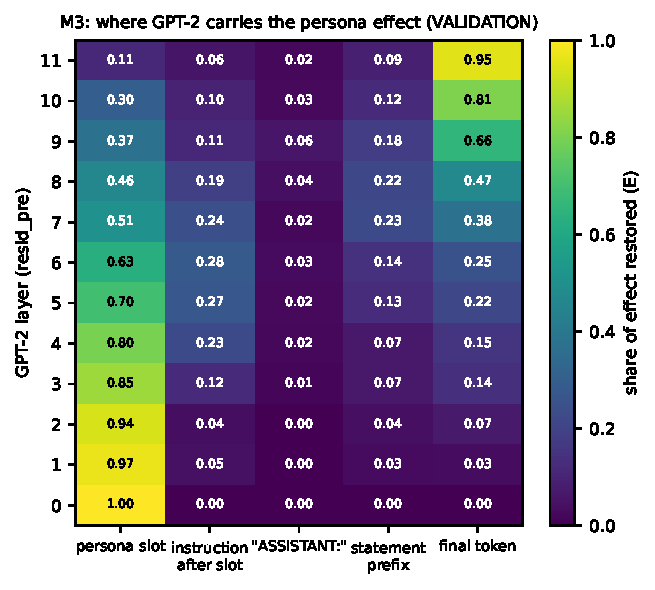
\includegraphics[width=0.62\linewidth]{fig_m3_sites}
  \caption{M3 (\evlabel{validation}): share of the persona-instruction effect restored by patching one position
  group at one layer of GPT-2 Small.}
  \label{fig:m3}
\end{figure}

\paragraph{How much of the effect the SAE carries (M4).} At a site, let $\Delta=x_H-x_U$, $\Delta_{\text{rec}}=\hat{x}_H-\hat{x}_U$
and $\Delta_{\text{err}}=e_H-e_U$, so $\Delta=\Delta_{\text{rec}}+\Delta_{\text{err}}$ exactly. With
$T(v)=\mathrm{KL}(p_H\|p_U)-\mathrm{KL}(p_H\|p_{U+v})$, we define $T_{\text{full}}=T(\Delta)$,
$T_{\text{rec}}=T(\Delta_{\text{rec}})$, $T_{\text{err}}=T(\Delta_{\text{err}})$, the interaction
$I=T_{\text{full}}-T_{\text{rec}}-T_{\text{err}}$, and Shapley shares $\phi_{\text{rec}}=(T_{\text{rec}}+T_{\text{full}}-T_{\text{err}})/2$.
The patch adds $v$ to the dishonest run's original activation; it is not a full splice. All exact checks pass
($\Delta$ identity error $9.5\times10^{-7}$; $T_{\text{full}}$ reproduces M3 to $7\times10^{-8}$).

Table~\ref{tab:m4} and Figure~\ref{fig:m4} show that the reconstructed difference restores 93--97\,\% of the effect at
the layer-1 persona token, but only 62--68\,\% at the layer-8 and layer-11 final token. There, ReLU's error part alone
carries 40--45\,\%; for TopK and JumpReLU, the interaction is large ($|I|/T_{\text{full}}$ 0.26--0.38), so their
shares cannot be read additively. The persona-minus-synonym difference is preserved in the reconstruction at every
site. Higher explained variance does not imply higher causal preservation: at layer 11, TopK has higher EV than ReLU
(0.815 vs 0.757) but keeps less of the effect (0.62 vs 0.68).

\paragraph{SAE-selected feature patches (error term kept).} Encoding both prompts, setting the dishonest prompt's top-$k$ features to
their honest values, decoding and keeping the error term restores more than 200 frequency- and magnitude-matched
random feature sets in all 27 SAE $\times$ site combinations ($p=0.005$, the minimum attainable). The effect is
distributed: one feature carries 2--10\,\% of $T_{\text{rec}}$ and 64 features 47--74\,\%. This shows that
SAE-defined directions are causally sufficient when inserted; it does not show that GPT-2 uses SAE features.

\paragraph{What these patches are, mathematically.} Because the error term is kept, every M4 patch has the form
$x_U+v$ with $v=W_{\text{dec}}(z'-z_U)$; the decoder bias cancels. $T_{\text{rec}}$ adds $v=W_{\text{dec}}(z_H-z_U)$
and the top-$k$ patch adds $W_{\text{dec},S}(z_{H,S}-z_{U,S})$. Each is therefore identical to adding one vector to
the dishonest prompt's raw activation. The same holds for any encode--edit--decode intervention that keeps the error,
including input-dependent clamps: $x'=x+W_{\text{dec}}(z'(x)-z(x))$. Because a dictionary of 3,072 or 12,288
latents spans $\mathbb{R}^{768}$, lying in decoder space does not restrict $v$. The only SAE-specific ingredient is how
$v$ is chosen: the encoder's input-dependent latent selection on the two prompts. The matched random-feature-set and
isotropic controls test that choice. The patches therefore establish that the SAE \emph{selects} input-dependent
directions that carry the effect when inserted. They do not establish an effect that is \emph{mediated} by the SAE,
which is what Review~\#8 asked of an SAE-in-the-loop intervention. Establishing mediation needs the downstream
computation to pass through SAE nonlinearities. Examples are an edit at layer $\ell$ with SAEs spliced at later
layers, or a run on $\hat{x}$ with no error term, compared against the spliced baseline. The layer-6 clamp
experiment (R2-clamp; input-dependent clamps, with and without the error term) found no supported effect
(\evlabel{validation}).

% generated by scripts/shared/build_paper_artifacts.py from results/repe/sae_patch_decomposition/architecture_summary.csv
\begin{table}[t]
\centering
\small
\caption{M4 causal decomposition (VALIDATION; templates T2--T4; mean$\pm$sd over 3 seeds). Shapley shares in parentheses are not interpretable as additive (pre-registered rule: interaction too large). Source: \texttt{results/\allowbreak{}repe/\allowbreak{}sae\_patch\_decomposition/\allowbreak{}architecture\_summary.csv}.}
\label{tab:m4}
\begin{adjustbox}{max width=\linewidth}
\begin{tabular}{llccccc}
\toprule
Site & SAE & $T_{\text{full}}$ (nats) & $T_{\text{rec}}/T_{\text{full}}$ & $T_{\text{err}}/T_{\text{full}}$ & $|I|/T_{\text{full}}$ & $\phi_{\text{rec}}$ \\
\midrule
L1 persona slot & ReLU & 0.0435 & 0.938$\pm$0.019 & 0.14 & 0.12 & 0.90 \\
 & TopK & 0.0435 & 0.931$\pm$0.014 & 0.16 & 0.14 & 0.89 \\
 & JumpReLU & 0.0435 & 0.968$\pm$0.011 & 0.03 & 0.10 & 0.97 \\
L8 final token & ReLU & 0.0220 & 0.621$\pm$0.015 & 0.45 & 0.12 & 0.59 \\
 & TopK & 0.0220 & 0.625$\pm$0.039 & 0.09 & 0.32 & (0.77) \\
 & JumpReLU & 0.0220 & 0.665$\pm$0.011 & 0.11 & 0.26 & (0.78) \\
L11 final token & ReLU & 0.0430 & 0.677$\pm$0.014 & 0.40 & 0.16 & 0.64 \\
 & TopK & 0.0430 & 0.620$\pm$0.004 & 0.06 & 0.38 & (0.78) \\
 & JumpReLU & 0.0430 & 0.678$\pm$0.007 & 0.11 & 0.28 & (0.78) \\
\bottomrule
\end{tabular}
\end{adjustbox}
\end{table}


\begin{figure}[t]
  \centering
  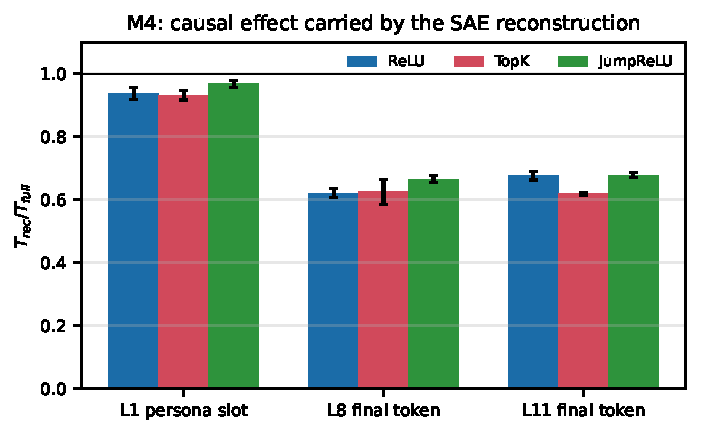
\includegraphics[width=0.62\linewidth]{fig_m4_preservation}
  \caption{M4 (\evlabel{validation}): share of the causal effect carried by the SAE-reconstructed activation
  difference ($T_{\text{rec}}/T_{\text{full}}$; mean$\pm$sd over 3 seeds; T2--T4).}
  \label{fig:m4}
\end{figure}

Whether fine-tuning changes this decomposition is tested in E3 (\S\ref{sec:e3}).

\pending{Minimum detectable effect statement (Review \#8 critique 3); M5 held-out confirmation.}
